\documentclass[11pt]{article}
\usepackage{amsmath, amscd, amssymb, amsthm}
% \usepackage{diagrams}
\usepackage{color}
\usepackage{graphicx, psfrag, tikz}
\usepackage[all]{xy}
\usepackage[margin=1.1in]{geometry}

\usepackage{enumitem,kantlipsum}


\newtheorem{theorem}{Theorem}[section]
\newtheorem{lemma}[theorem]{Lemma} 
\newtheorem{proposition}[theorem]{Proposition}
\newtheorem{corollary}[theorem]{Corollary}
\theoremstyle{definition} 
\newtheorem{definition}[theorem]{Definition}
\newtheorem{conjecture}[theorem]{Conjecture}
\newtheorem{remark}[theorem]{Remark}
\newtheorem{example}[theorem]{Example}

\begin{document}
\begin{center}
\textbf{Math 309 Homework 1}\\
(8 problems)
\end{center}
\vspace{0.2in}


\noindent \textbf{Reminder:}  Solutions should be presented using complete sentences, with grammatically correct English, that combine both words and precise mathematical expressions to articulate your line of reasoning.  Collaboration on homework is encouraged, but you need to write up the solutions in your own words that reflect your own understanding of the material. 



\begin{enumerate}[leftmargin=*]

\item (a) Find a nonzero matrix $A$ such that $A^2=0$.\\
(b) Find a square matrix $P$, other than the zero matrix and the identity matrix, such that $P^2=P$.

\item For parts (a) and (b), determine wether the members of the given set of vectors are linearly independent, and explain your reason.  If they are linearly dependent, find a linear relation among them.\\

(a) $x^{(1)} = \left[
\begin{array}{c}
1\\
1
\end{array}\right] 
$, $x^{(2)} = \left[
\begin{array}{c}
0\\
1
\end{array}\right],
$
$x^{(3)} = \left[
\begin{array}{c}
1\\
0
\end{array}\right];
$\\

(b) $x^{(1)} = \left[
\begin{array}{c}
2\\
1\\
0
\end{array}\right] 
$, $x^{(2)} = \left[
\begin{array}{c}
0\\
1\\
0
\end{array}\right],
$
$x^{(3)} = \left[
\begin{array}{c}
-1\\
2\\
0
\end{array}\right].
$\\

(c) Find all constant solutions $x(t)=
\left[
\begin{array}{c}
x_1(t)\\
x_2(t)\\
x_3(t)
\end{array}\right]$ (i.e. $x_1, x_2, x_3$ are actually constant functions) to the following system of differential equations
\[
x'=
\left[
\begin{array}{ccc}
2&0 & -1\\
1&1 &2\\
0 & 0& 0
\end{array}\right]x.
\]
Note that the columns of this matrix is the same as the three vectors in part (b).  \emph{Hint: what is $x'(t)$ when $x(t)$ is constant? }

\item Find all eigenvalues and eigenvectors of the matrix
$ 
\left[
\begin{array}{cc}
3&-2\\
4&-1
\end{array}\right].
$
\item Find all eigenvalues and eigenvectors of the matrix
$ 
\left[
\begin{array}{ccc}
1&0&0\\
2&1&-2\\
3&2&1
\end{array}\right].
$\\


\item Consider the matrix $\left[
\begin{array}{ccc}
1&-1&1\\
0&3&0\\
0&0&3
\end{array}\right].$
Find the set of eigenvectors corresponding to the eigenvalue $\lambda=3$.

\item Let $M$ be a $2\times 2$ matrix that has only one real eigenvalue (i.e. the two eigenvalues are the same) and the set of eigenvectors corresponding to the eigenvalue has dimension 2.  Show that $M$ must be a diagonal matrix with diagonal entires being the eigenvalue. 

\item Verify that the vector 
\[
x=\left[
\begin{array}{c}
1\\
0
\end{array}\right] e^t+ 2\left[
\begin{array}{c}
1\\
1
\end{array}\right] te^t
\]
satisfies the differential equation
\[x'=\left[
\begin{array}{cc}
2&-1\\
3&-2
\end{array}\right] x+ \left[
\begin{array}{c}
1\\
-1
\end{array}\right]e^t.
 \]
 
 \item (Pendulum) A pendulum of length $L$ is hanging from the ceiling.  Neglect air resistance and assume that the mass of the rod is negligible and the mass of the bob is $m$. 

There are two forces acting on the bob of the pendulum, the tension from the rod and the force due to gravity.   The force due to gravity is a downward force of magnitude $mg$, which can be resolved into two components as illustrated in the figure below.  One component is directly opposite of and balanced out by the tension from the string.  The other component that is perpendicular to the string is the force that causes motion, and the magnitude of this component is $mg\sin \theta$.
\begin{center}
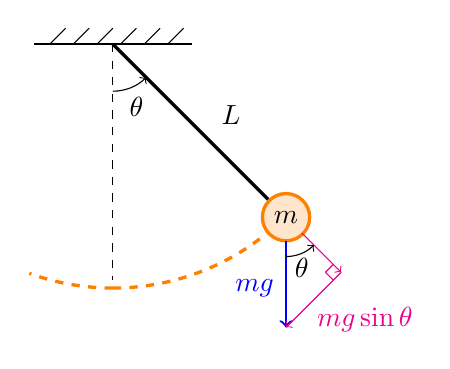
\begin{tikzpicture}
 \draw  (-1, 0) -- (1, 0);
 \draw  (-0.8, 0)--(-0.6, 0.2);
 \draw  (-0.5, 0)--(-0.3, 0.2);
 \draw  (-0.2, 0)--(-0, 0.2);
 \draw  (0.1, 0)--(0.3, 0.2);
 \draw  (0.4, 0)--(0.6, 0.2);
 \draw  (0.7, 0)--(0.9, 0.2);
 
 \draw [dashed] (0,0) -- (0, -3);
 \draw[very thick] (0,0)--(2,-2);
 \draw[orange, very thick,fill=orange!20] (2.2, -2.2) circle (0.3cm);
 \draw [->](0,-0.6) arc (-90:-45:0.6);
 \node at (0.3, -0.8) {$\theta$};
  \node at (1.5, -0.9) {$L$};
  \node at (2.2, -2.2) {$m$};
     
     
 \draw[->, blue, thick] (2.2, -2.5) -- (2.2, -3.6);
 \draw[->, magenta ](2.4, -2.4) -- (2.9, -2.9);
  \draw[->, magenta](2.9, -2.9) -- (2.2, -3.6);
  \draw[magenta] (2.8,-2.8) --(2.7, -2.9);
    \draw[magenta] (2.7,-2.9) --(2.8, -3);
    
   \draw [->](2.2,-2.7) arc (-90:-45:0.5);
   \node at (2.4, -2.85) {$\theta$};
   \node at (1.8, -3.1) {\textcolor{blue}{$mg$}};
    \node at (3.2, -3.5) {\textcolor{magenta}{$mg\sin \theta$}};
          
  \draw[dashed, orange, very thick] (0, -3.1) arc (-90:-51: 3.1);
    \draw[dashed, orange, very thick] (0, -3.1) arc (-90: -110: 3.1);
\end{tikzpicture}
\end{center}

The trajectory of the bob is an arc of a circle of radius $L$, so its position can be described by $L\theta(t)$.  Newton's equation of motion for the bob is then
\[
m \frac{d^2(L\theta(t))}{dt^2}= - mg\sin \theta.
\]
(Note the $-$ sign is there because the force is in the direction that decreases $\theta$).  Simplifying the above equation gives 
\[
\frac{d^2\theta(t)}{dt^2}=-\frac{g}{L}\sin \theta.
\]
Note that $g$ and $L$ are constants, and this is a 2nd order differential equation in $\theta(t)$.

(a) Denote by  $\omega(t)=\frac{d\theta(t)}{dt}$.  Write the above 2nd order equation as a system of first order equations  in $\theta$ and $\omega$ in the following form
\[
\begin{cases}
\theta'=\\
\omega'= 
\end{cases},
\]
where the right hand side are functions of $\theta$ and $\omega$ (no derivatives on the right hand side).  

(b) Note that the equation above is a nonlinear equation because $\sin\theta$ is a not a linear function of $\theta$.  When $\theta$ is small, we can approximate $\sin \theta\approx \theta$, then the equation above becomes 
\[
\frac{d^2\theta(t)}{dt^2}=-\frac{g}{L}\theta.
\]
This is a linear equation.  It is also a 2nd order homogeneous equation with constant coefficients.  Find the general solution for $\theta(t)$.  After that, differentiate $\theta(t)$ to find the general formula for $\omega(t)$.

(c) Write the linear equation $\frac{d^2\theta(t)}{dt^2}= -\frac{g}{L}\theta$ as a system of first order equations in $\theta$ and $\omega$,
\[
\begin{cases}
\theta'=\\
\omega'= 
\end{cases}.
\]
After that, write this system in the matrix form
\[
\left[\begin{array}{l} \theta'\\ \omega' \end{array}\right]=A  \left[\begin{array}{l} \theta \\ \omega \end{array}\right],
\]
where $A$ is a $2\times 2$ matrix.

 
 
 
\end{enumerate}
 
 \end{document}




